\documentclass{article}

% Language setting
% Replace `english' with e.g. `spanish' to change the document language
\usepackage[english]{babel}

% Set page size and margins
% Replace `letterpaper' with `a4paper' for UK/EU standard size
\usepackage[letterpaper,top=2cm,bottom=2cm,left=3cm,right=3cm,marginparwidth=1.75cm]{geometry}
\usepackage{CJKutf8}
% Useful packages
\usepackage{amsmath}
\usepackage{graphicx}
\usepackage{setspace}
\usepackage{float}
\usepackage{subfigure}
\usepackage[section]{placeins}
\usepackage[colorlinks=true, allcolors=blue]{hyperref}
\usepackage[export]{adjustbox}
\usepackage{array}

\author{B10209040 陳彥倫}

\begin{document}
\thispagestyle{empty}
\hfill {\scshape \large Statistics with Meteorological Applications, Spring 2024} \hfill {\scshape P1}
\smallskip
\hrule
\begin{CJK*}{UTF8}{bsmi}
\bigskip
\bigskip
\bigskip

\centerline{\huge \textbf {HW7}}
\bigskip
\centerline{\textbf {B10209040 陳彥倫}}

\bigskip
\bigskip
\bigskip

\section*{7.1}
    \begin{spacing}{2.5}
        \begin{large}
            \begin{center}
                Explanatory variable(X): Temperature of Taipei\\
                Responce variable(Y): Temperature of Hengchun
            \end{center}
        \end{large}
    \end{spacing}

\section*{7.2}
    \subsection*{}
        \begin{figure}[htbp]
            \centering
            \begin{minipage}[t]{0.7\textwidth}
                \centering
                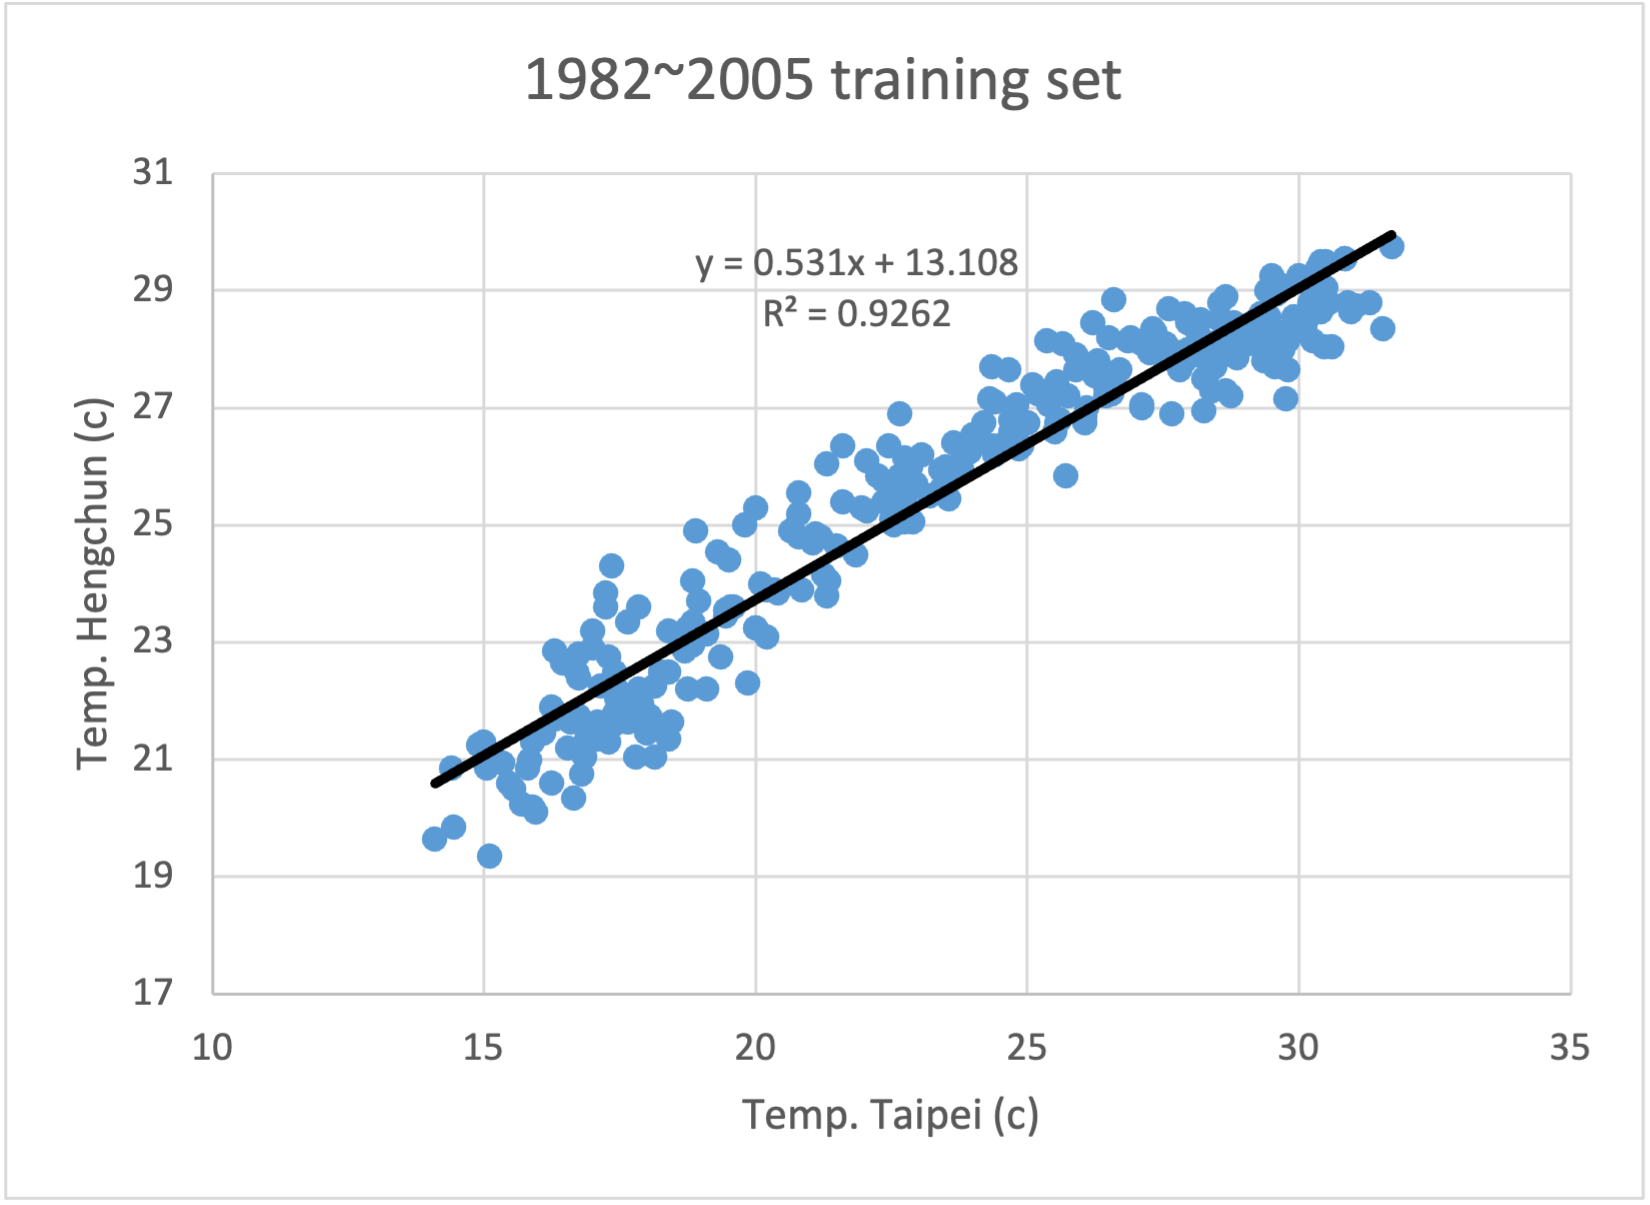
\includegraphics[width=10.5cm]{Picture1.png}
                \caption{scatter plot}
                \end{minipage}
        \end{figure}

\newpage
\thispagestyle{empty}
\hfill {\scshape \large Statistics with Meteorological Applications, Spring 2024} \hfill {\scshape P2}
\smallskip
\hrule
\bigskip
\bigskip
\bigskip

    \subsection*{}
        \begin{figure}[h]
            \begin{minipage}{0.5\textwidth}
                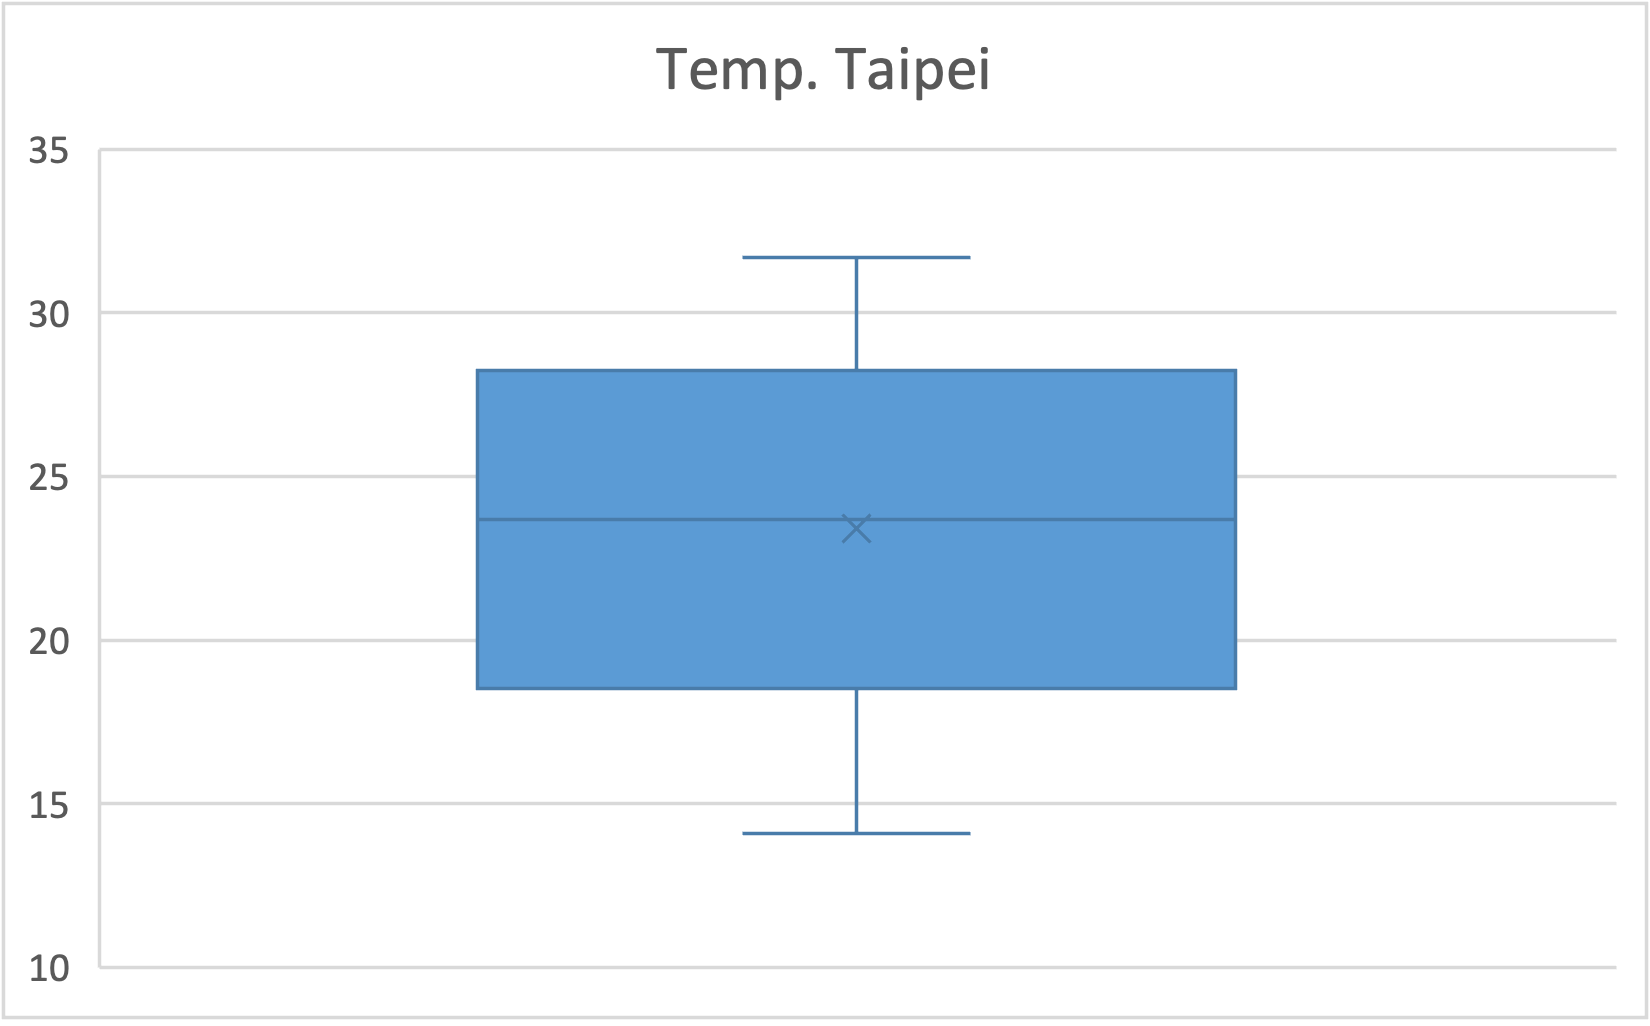
\includegraphics[width=7.6cm]{Picture2.png} 
                \label{fig:subim1}
            \end{minipage}
                \begin{minipage}{0.5\textwidth}
                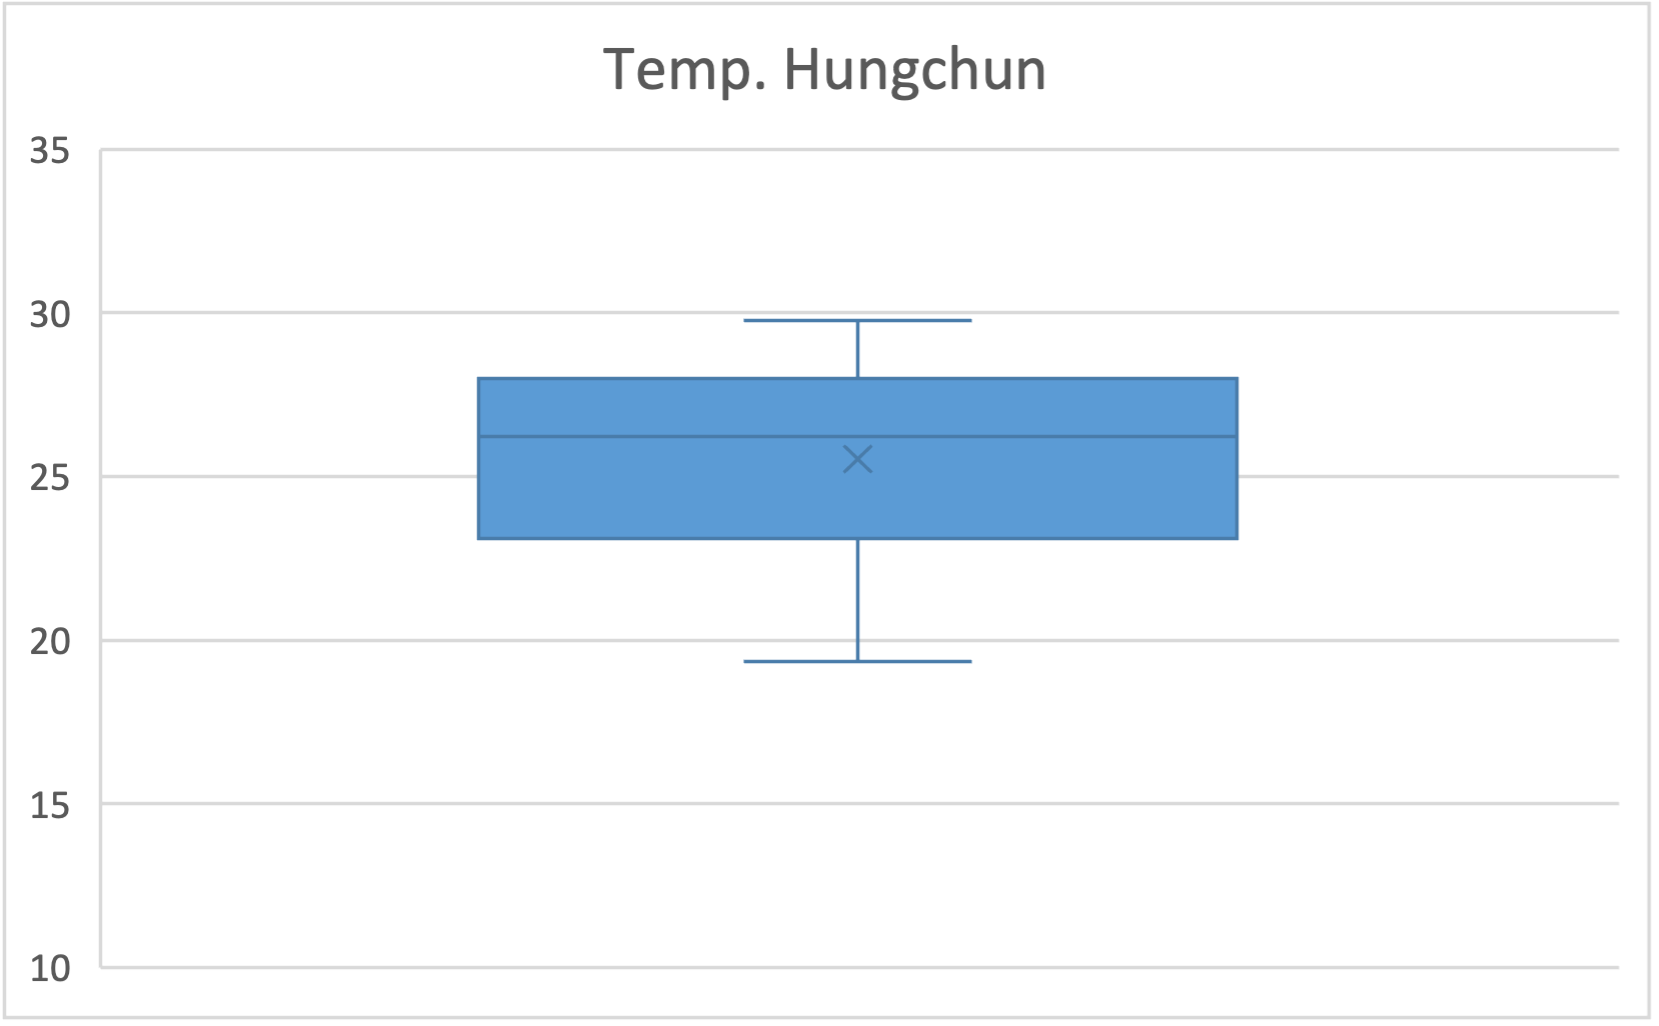
\includegraphics[width=7.6cm]{Picture3.png}
                \label{fig:subim2}
            \end{minipage}
            \caption{box plot of Taipei and Hengchen}
        \end{figure}
    
        \subsection*{}
        \begin{spacing}{2.5}
            \begin{large}
                由散佈圖可以看出資料點有集中在一條斜直線上的趨勢,表示同一時間點北部跟南部的氣溫高低存在一定的關聯性。
                而箱型圖則是告訴我們兩個測站氣溫資料的分布情形,左圖顯示台北的最高月均溫高於恆春、最低月均溫也低於恆春,
                表示氣溫分布較極端,但平均溫度恆春地區仍高於台北。
            \end{large}
        \end{spacing}


\section*{7.3}
\begin{spacing}{2.5}
    \begin{large}
        \begin{center}
            y = 0.531x + 13.108 \\
            相關係數:0.9624 \\
            $R^2$ = 0.9262
        \end{center}
    \end{large}
\end{spacing}

\newpage
\thispagestyle{empty}
\hfill {\scshape \large Statistics with Meteorological Applications, Spring 2024} \hfill {\scshape P3}
\smallskip
\hrule
\bigskip
\bigskip
\bigskip

\section*{7.4}
\begin{spacing}{2.5}
    \begin{large}
            $R^2$ 的數值為相關係數的平方,表示7.2的迴歸模型中解釋了約93\%的變異,相當接近100\%表示資料點很符合迴歸直線。
    \end{large}
\end{spacing}

\section*{7.5}
\begin{spacing}{2.5}
    \begin{large}
        \subsection*{}
        \begin{figure}[htbp]
            \centering
            \begin{minipage}[t]{0.7\textwidth}
                \centering
                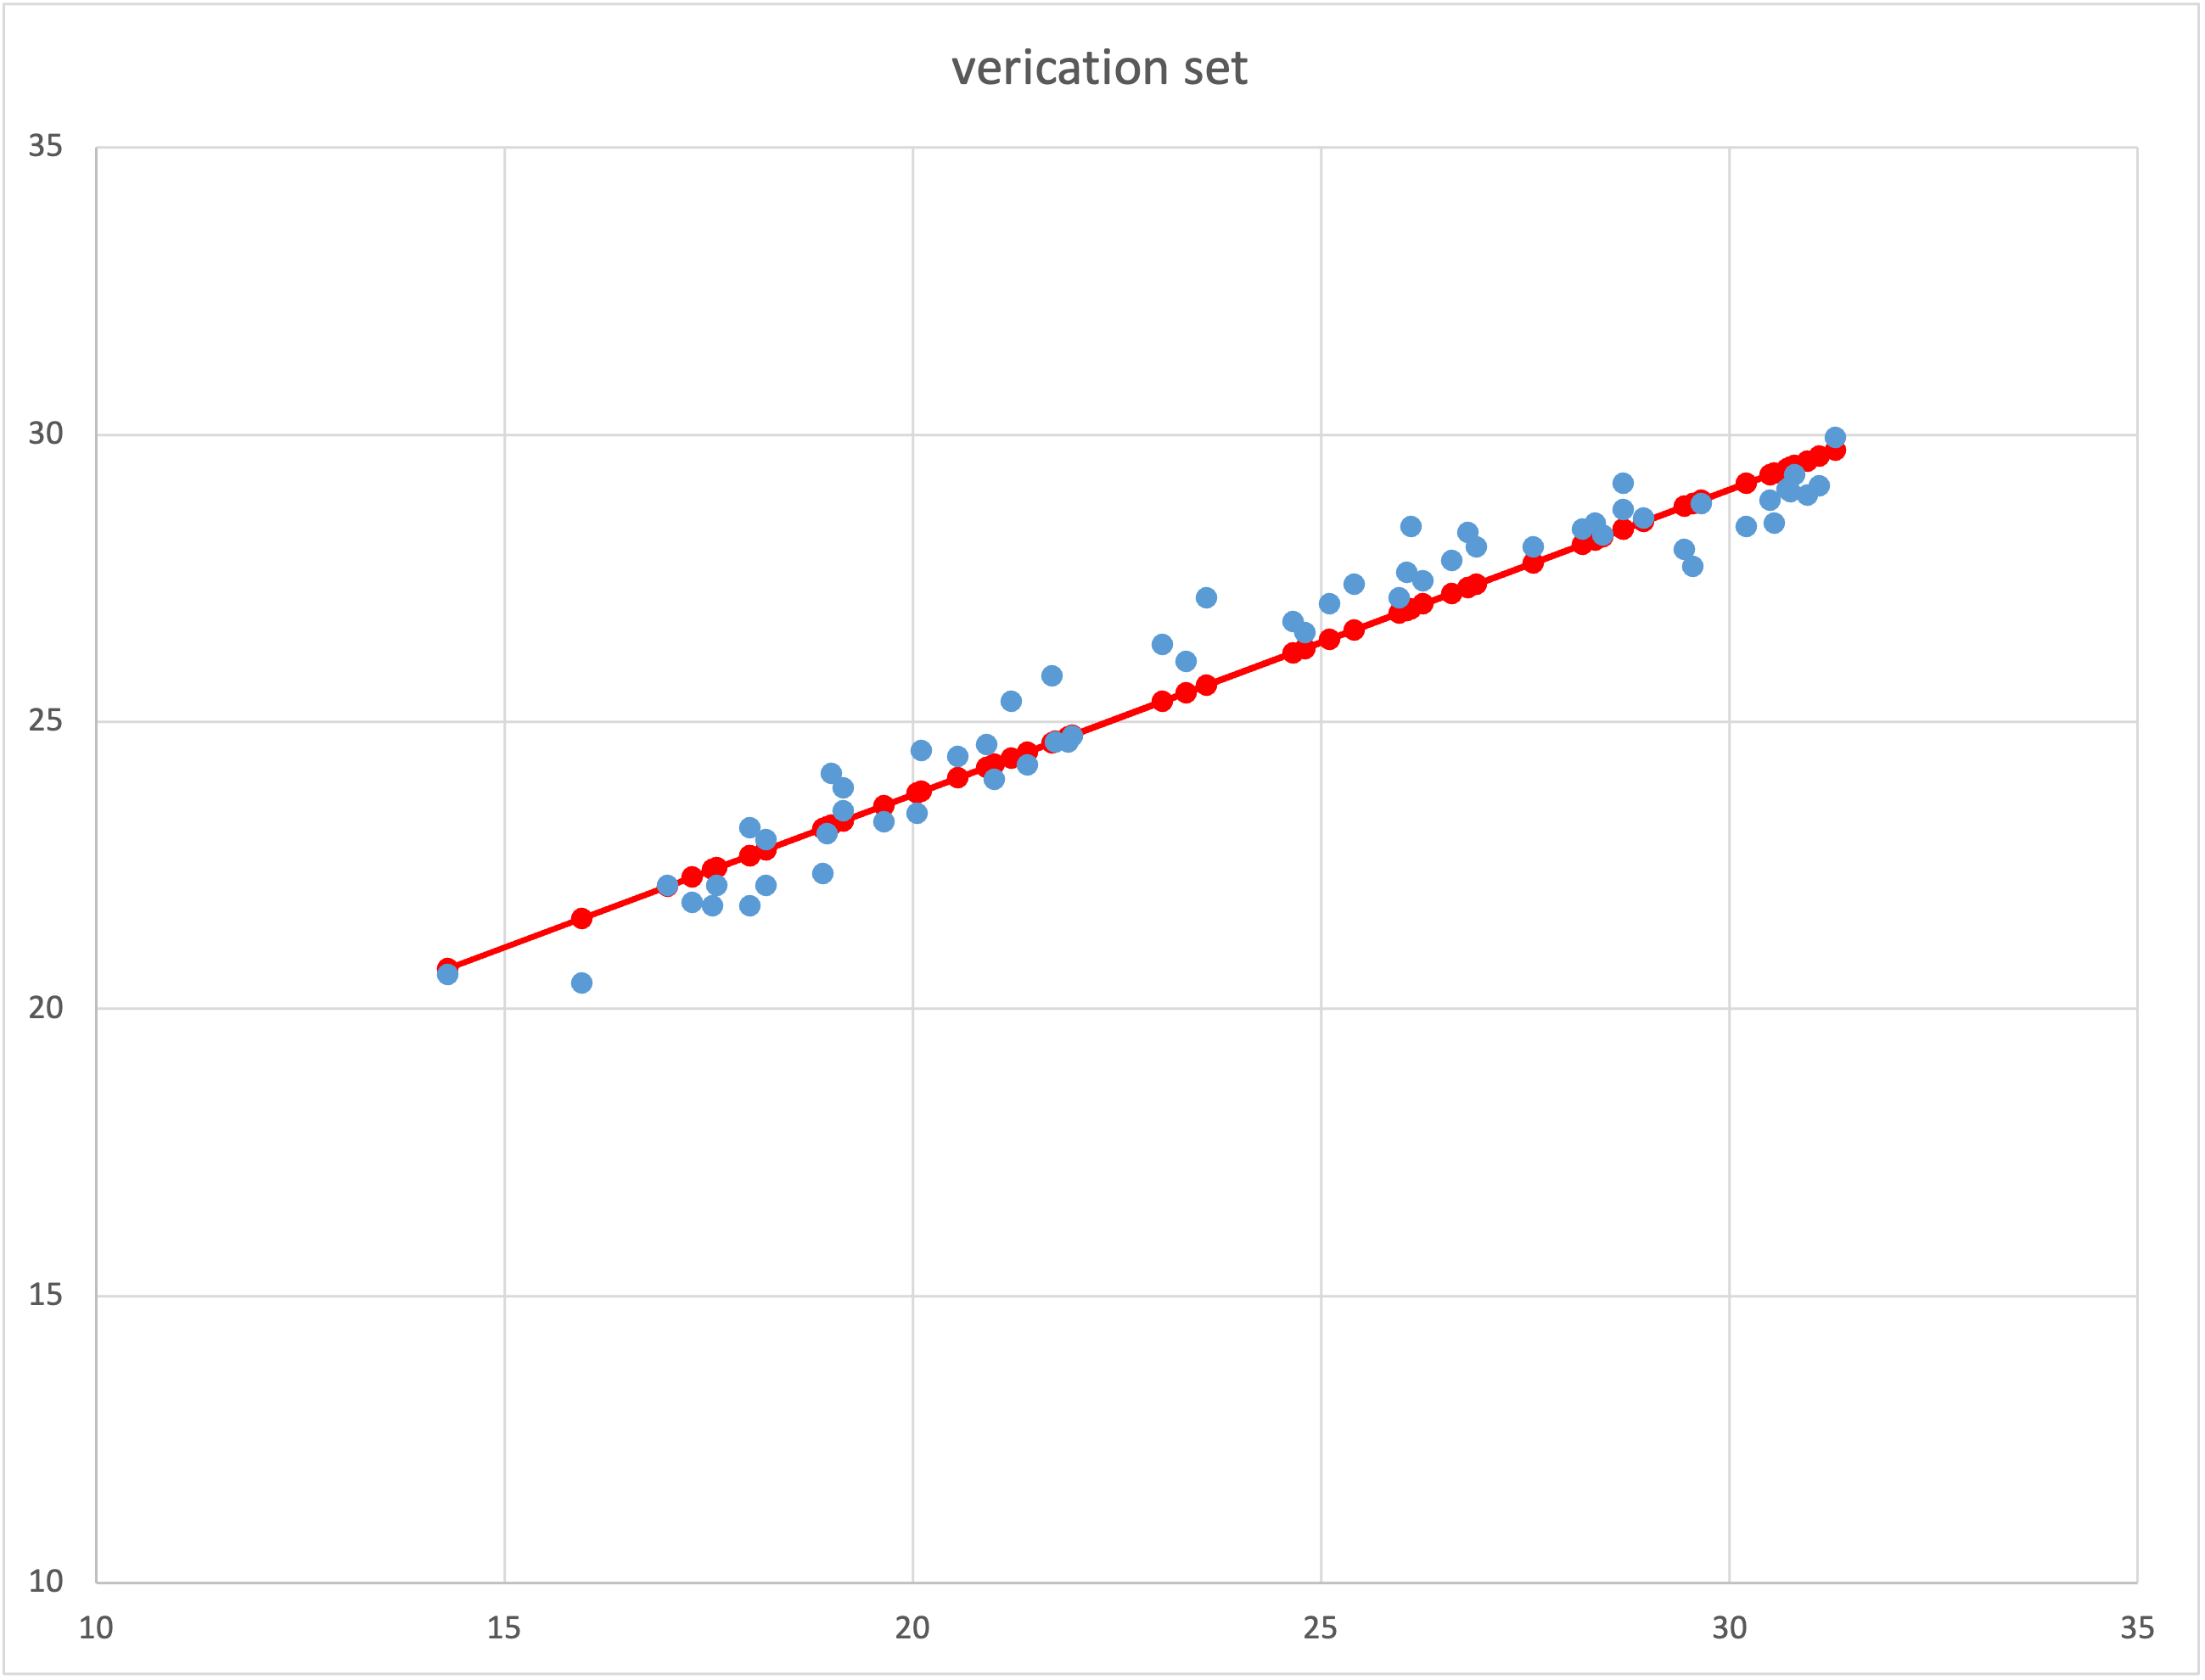
\includegraphics[width=10.5cm]{Picture4.png}
                \caption{red line: the result of regression model in 7.3}
                \end{minipage}
        \end{figure}

        \subsection*{}

    \end{large}
\end{spacing}

\newpage
\thispagestyle{empty}
\hfill {\scshape \large Statistics with Meteorological Applications, Spring 2024} \hfill {\scshape P4}
\smallskip
\hrule
\bigskip
\bigskip
\bigskip

\subsection*{}
\begin{spacing}{2.5}
    \begin{large}
        將2006年至2010年台北測站的氣溫帶入前述計算的regression model,可以得到Figure.3的紅點分布,
        走向與實際恆春氣溫大致符合。若計算每個時間點的residual,即模型輸出的值與實際值的差距,平均約為
        -0.1042。若與真實平均氣溫相比,誤差比例約為2.7\% 。
    \end{large}
\end{spacing}

\end{CJK*}
\end{document}